\documentclass[12pt]{article}
% \usepackage[top=1in,left=1in, right = 1in, footskip=1in]{geometry}
\usepackage[top=1in,footskip=1in]{geometry}

\usepackage{graphicx}
\usepackage{xspace}
%\usepackage{adjustbox}

\usepackage{multirow}
\usepackage{booktabs}

\usepackage{pdflscape}

\usepackage{grffile}

\newcommand{\comment}{\showcomment}
%% \newcommand{\comment}{\nocomment}

\newcommand{\showcomment}[3]{\textcolor{#1}{\textbf{[#2: }\textsl{#3}\textbf{]}}}
\newcommand{\nocomment}[3]{}

\newcommand{\jd}[1]{\comment{cyan}{JD}{#1}}
\newcommand{\swp}[1]{\comment{magenta}{SWP}{#1}}
\newcommand{\bmb}[1]{\comment{blue}{BMB}{#1}}
\newcommand{\djde}[1]{\comment{red}{DJDE}{#1}}

\newcommand{\eref}[1]{Eq.~(\ref{eq:#1})}
\newcommand{\fref}[1]{Fig.~\ref{fig:#1}}
\newcommand{\Fref}[1]{Fig.~\ref{fig:#1}}
\newcommand{\sref}[1]{Sec.~\ref{#1}}
\newcommand{\frange}[2]{Fig.~\ref{fig:#1}--\ref{fig:#2}}
\newcommand{\tref}[1]{Table~\ref{tab:#1}}
\newcommand{\tlab}[1]{\label{tab:#1}}
\newcommand{\seminar}{SE\mbox{$^m$}I\mbox{$^n$}R}

\usepackage{amsthm}
\usepackage{amsmath}
\usepackage{amssymb}
\usepackage{amsfonts}
\usepackage[utf8]{inputenc} % make sure fancy dashes etc. don't get dropped

\usepackage{lineno}
\linenumbers

\usepackage[pdfencoding=auto, psdextra]{hyperref}

\usepackage{natbib}
\bibliographystyle{unsrt}
\date{\today}

\usepackage{xspace}
\newcommand*{\ie}{i.e.\@\xspace}

\usepackage{color}

\newcommand{\Rx}[1]{\ensuremath{{\mathcal R}_{#1}}\xspace} 
\newcommand{\RR}{\ensuremath{{\mathcal R}}\xspace}
\newcommand{\Rres}{\Rx{\mathrm{res}}}
\newcommand{\Rinv}{\Rx{\mathrm{inv}}}
\newcommand{\Rhat}{\ensuremath{{\hat\RR}}}
\newcommand{\Rt}{\ensuremath{{\mathcal R}(t)}\xspace}
\newcommand{\tsub}[2]{#1_{{\textrm{\tiny #2}}}}
\newcommand{\dd}[1]{\ensuremath{\, \mathrm{d}#1}}
\newcommand{\dtau}{\dd{\tau}}
\newcommand{\dx}{\dd{x}}
\newcommand{\dsigma}{\dd{\sigma}}

\newcommand{\rx}[1]{\ensuremath{{r}_{#1}}\xspace} 
\newcommand{\rres}{\rx{\mathrm{res}}}
\newcommand{\rinv}{\rx{\mathrm{inv}}}

\newcommand{\psymp}{\ensuremath{p}} %% primary symptom time
\newcommand{\ssymp}{\ensuremath{s}} %% secondary symptom time
\newcommand{\pinf}{\ensuremath{\alpha_1}} %% primary infection time
\newcommand{\sinf}{\ensuremath{\alpha_2}} %% secondary infection time

\newcommand{\psize}{{\mathcal P}} %% primary cohort size
\newcommand{\ssize}{{\mathcal S}} %% secondary cohort size

\newcommand{\gtime}{\tau_{\rm g}} %% generation interval
\newcommand{\gdist}{g} %% generation-interval distribution
\newcommand{\idist}{\ell} %% incubation-period distribution

\newcommand{\total}{{\mathcal T}} %% total number of serial intervals

\usepackage{lettrine}

\newcommand{\dropcapfont}{\fontfamily{lmss}\bfseries\fontsize{26pt}{28pt}\selectfont}
\newcommand{\dropcap}[1]{\lettrine[lines=2,lraise=0.05,findent=0.1em, nindent=0em]{{\dropcapfont{#1}}}{}}

\begin{document}

\section*{Supplementary Materials}

\begin{flushleft}{
	\Large
	\textbf\newline{
	  Delayed introduction, contact variation, and susceptible dynamics explain spatial asynchrony during Korea's large pertussis outbreak
	}
}
\newline
\\
Sang Woo Park\textsuperscript{1,*}
\\
\bigskip
\textbf{1} School of Biological Sciences, Seoul National University, Seoul, Korea
\bigskip

*Corresponding author: sangwoopark@snu.ac.kr
\end{flushleft}

\section*{Supplementary Text}

\subsection*{S1 Stochastic simulation}

I considered a stochastic version of the SEIR model:
\begin{align}
\beta (t) &= \mathcal R_0 (1-\exp(-\gamma\Delta t)) \delta(t)\\
\textrm{FOI}(t) &= \frac{\beta (t) I_m(t-\Delta t)}{N_m}\\
\Delta S_m(t) &\sim \mathrm{Binomial}\left(S_m(t-\Delta t), 1- \exp(-\textrm{FOI}(t) \Delta t)\right) \\
\Delta E_m(t) &\sim \mathrm{Binomial}\left(E_m(t-\Delta t), 1- \exp(-\sigma \Delta t)\right)\\
\Delta I_m(t) &\sim \mathrm{Binomial}\left(I_m(t-\Delta t), 1- \exp(-\gamma \Delta t)\right)\\
S_m(t) &= S(t-\Delta t) -\Delta S_m(t)\\
E_m(t) &= E(t-\Delta t) -\Delta E_m(t) + \Delta S_m(t)\\
I_m(t) &= I(t-\Delta t) -\Delta I_m(t) + \Delta E_m(t)
\end{align}

\pagebreak

\section*{Supplementary Figure}

\setcounter{figure}{0}
\renewcommand{\thefigure}{S\arabic{figure}}

\begin{figure}[!th]
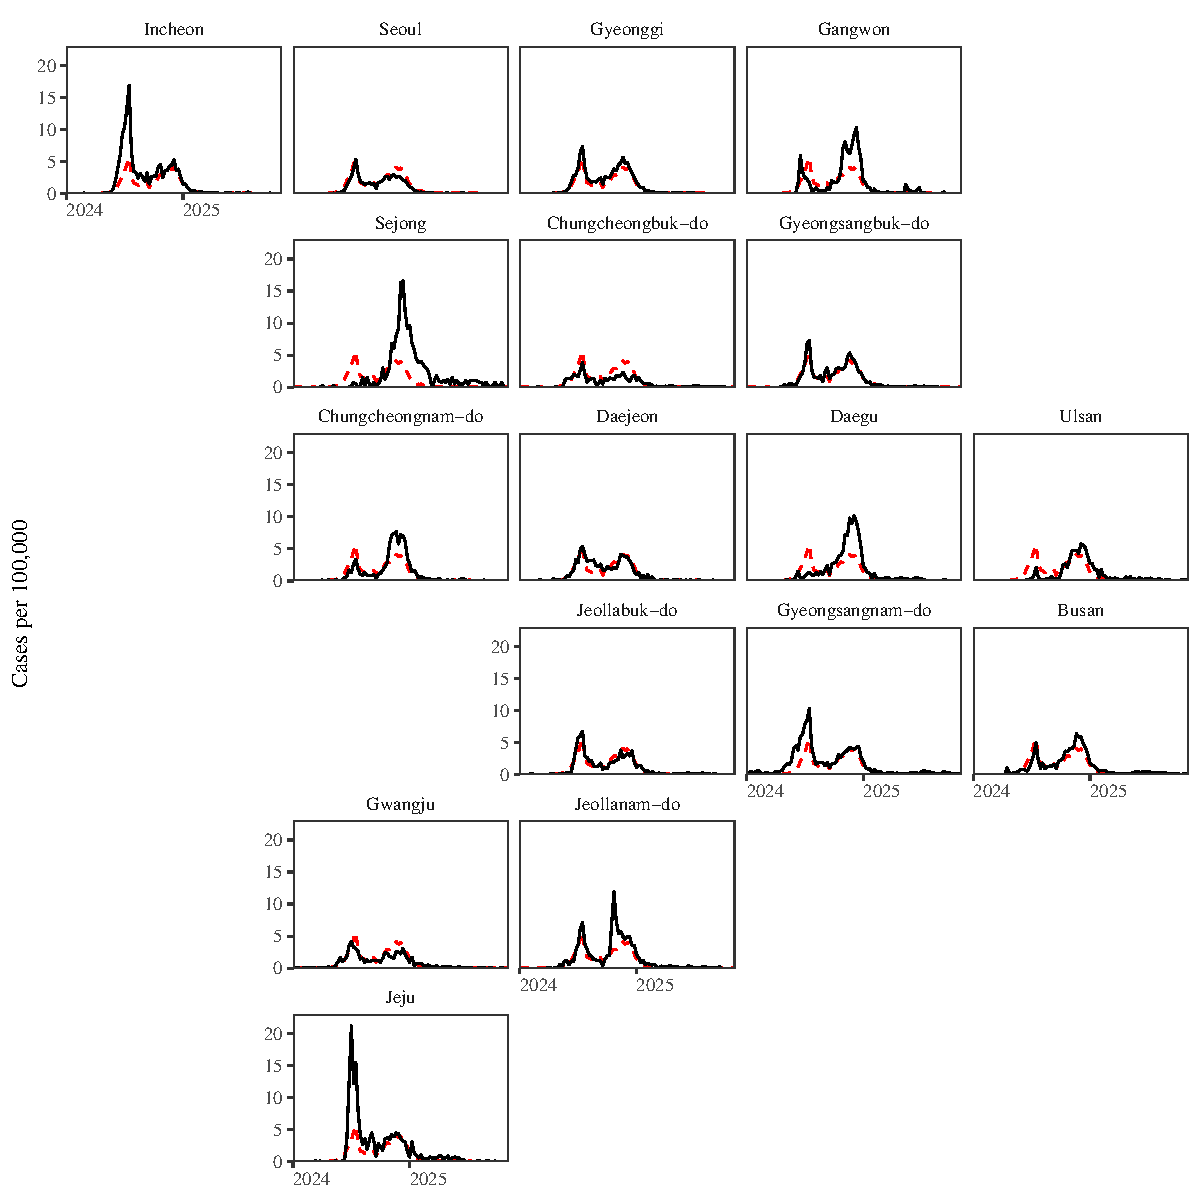
\includegraphics[width=\textwidth]{../figure/figure_data_region.pdf}
\caption{
\textbf{Spatiotempordal dynamics of pertussis outbreak in Korea across first-level administrative divisions, 2024---2025.}
Time series are arranged based on their approximate locations.
}
\end{figure}

\pagebreak

\begin{figure}[!th]
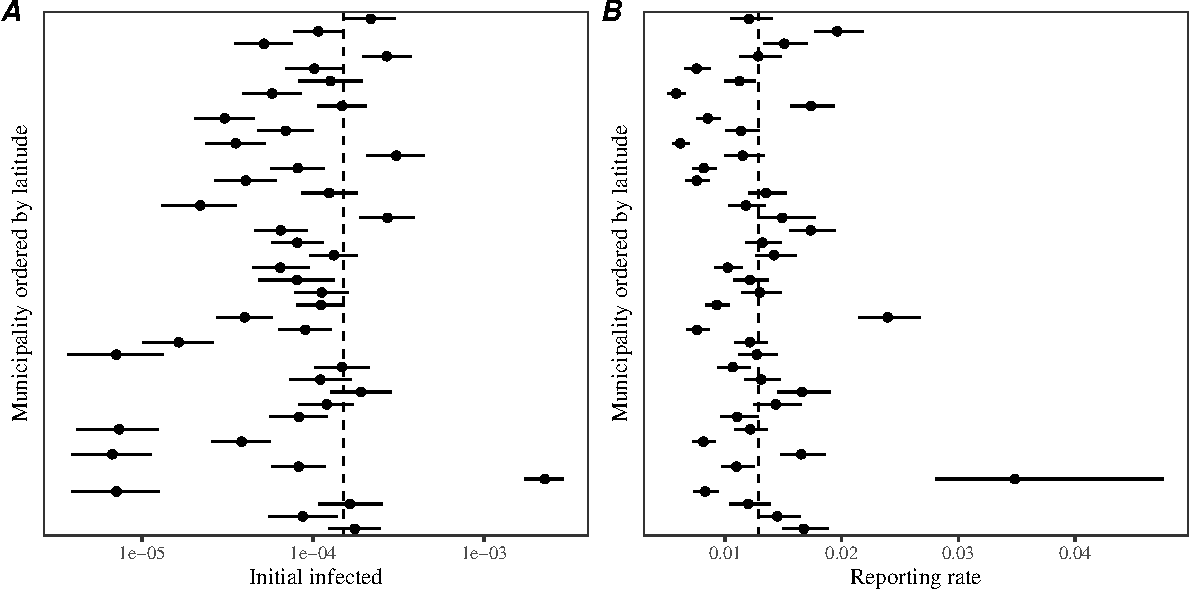
\includegraphics[width=\textwidth]{../figure/figure_stanfit_region_R0_supp_1.pdf}
\caption{
\textbf{Estimated initial infected fraction (A) and reporting rates (B) using time series data from municipalities with less than 400 total cases.}
Points represent posterior medians.
Error bars represent 95\% credible intervals.
}
\end{figure}

\pagebreak

\begin{figure}[!th]
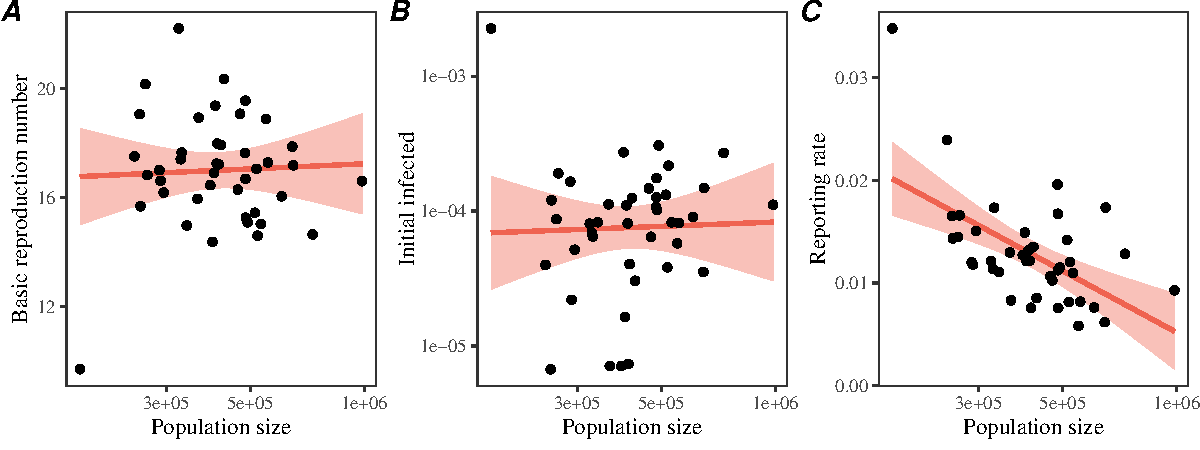
\includegraphics[width=\textwidth]{../figure/figure_stanfit_region_R0_supp_2.pdf}
\caption{
\textbf{Relationship between population size and parameter estimates for the basic reproduction number (A), initial infected fraction (B), and reporting rate (C).}
Points represent posterior medians.
Error bars represent 95\% credible intervals.
Red lines and shaded regions represent the linear regression fit and associated 95\% confidence intervals.
}
\end{figure}

\pagebreak

\begin{figure}[!th]
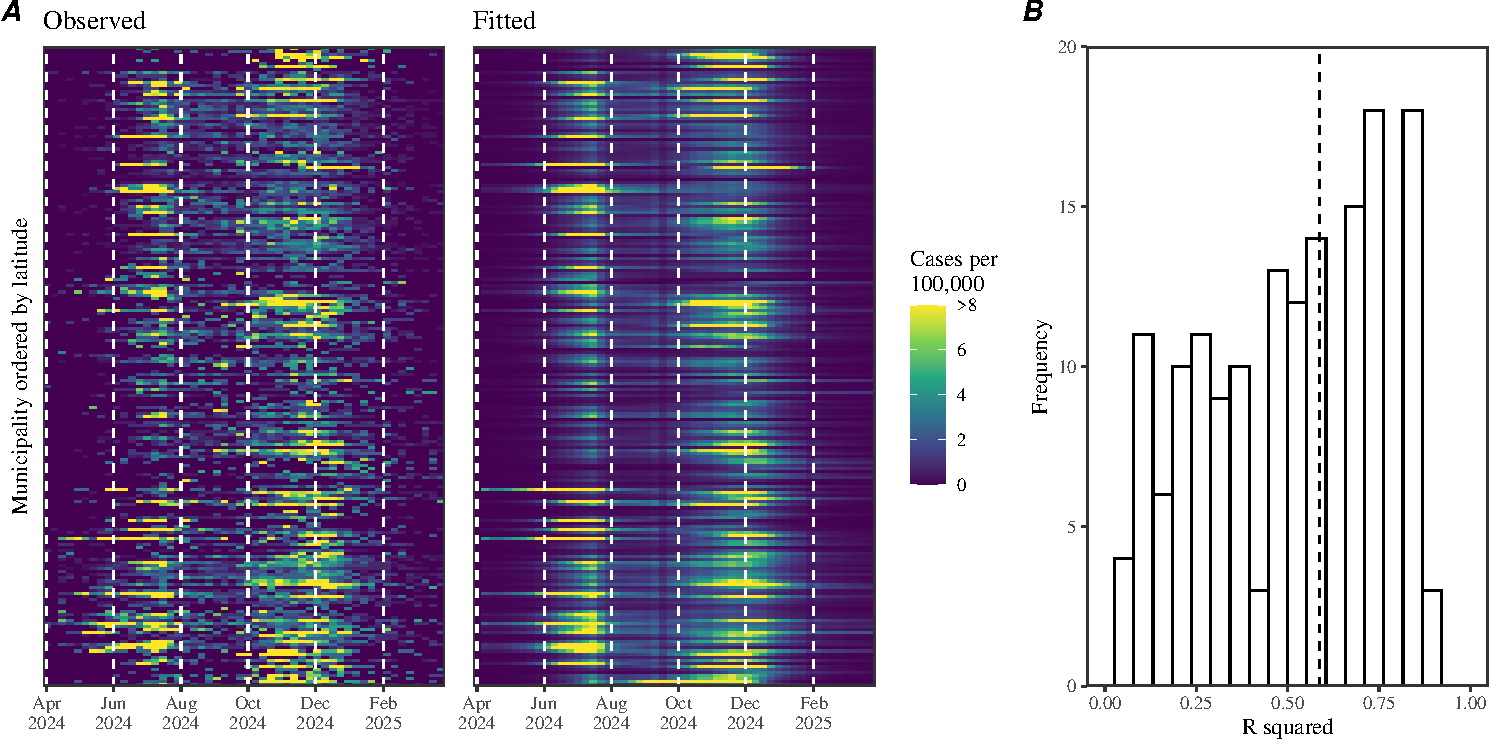
\includegraphics[width=\textwidth]{../figure/figure_stanfit_all_R0_delta.pdf}
\caption{
\textbf{Validation of the transmission model using time series data from municipalities with less than 400 total cases.}
(A) Comparisons between the observed and predicted epidemic dynamics across municipalities with less than 400 total cases, ordered by latitude.
(B) The bar plot represents the distribution of R squared values for model fits.
The vertical dashed line represents the median.
Initial infected, initial susceptible, basic reproduction number, and reporting probability were estimated for each region while assuming a known transmission variation term $\delta(t)$.
}
\end{figure}

\pagebreak

\begin{figure}[!ht]
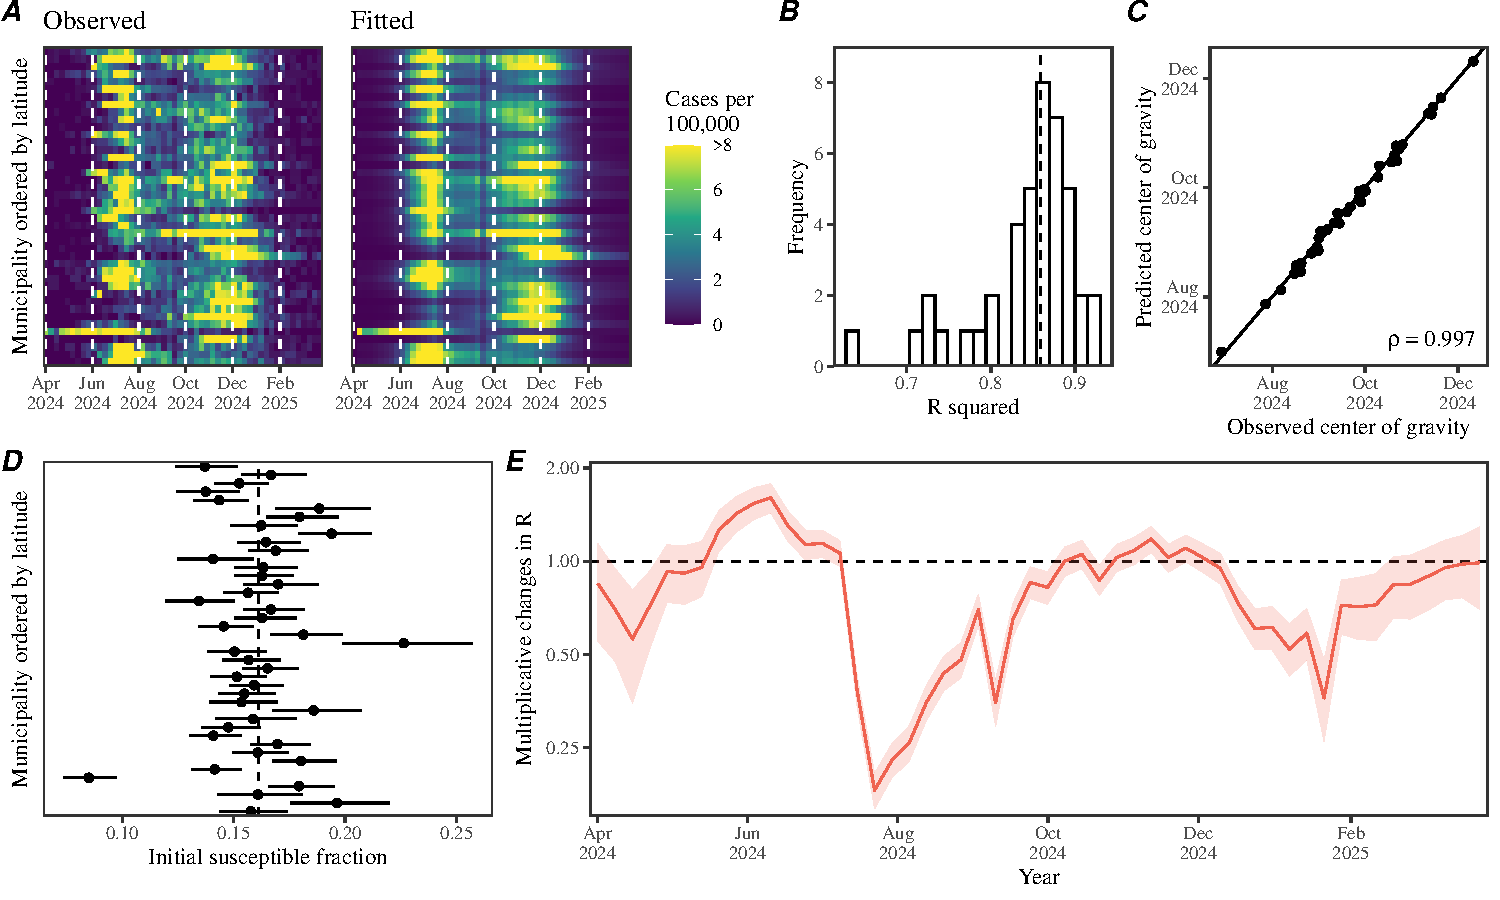
\includegraphics[width=\textwidth]{../figure/figure_stanfit_region.pdf}
\caption{
\textbf{Alternative SEIR model fits assuming variation in initial susceptible fraction.}
(A) Comparisons between the observed and predicted epidemic dynamics across municipalities with more than 400 total cases, ordered by latitude.
(B) The bar plot represents the distribution of R squared values for model fits.
The vertical dashed line represents the median.
(C) Relationship between the estimated and predicted center of gravity.
The solid line indicated the one-to-one relationship.
(D) Estimated initial susceptible fraction $S(0)$ across municipalities, ordered by latitude.
Points and error bars represent posterior medians and corresponding 95\% credible intervals.
(E) Estimated time-varying pertussis transmission multiplier.
The red line and shaded regions represent the posterior median and the corresponding 95\% credible interval.
}
\end{figure}

\pagebreak

\begin{figure}[!th]
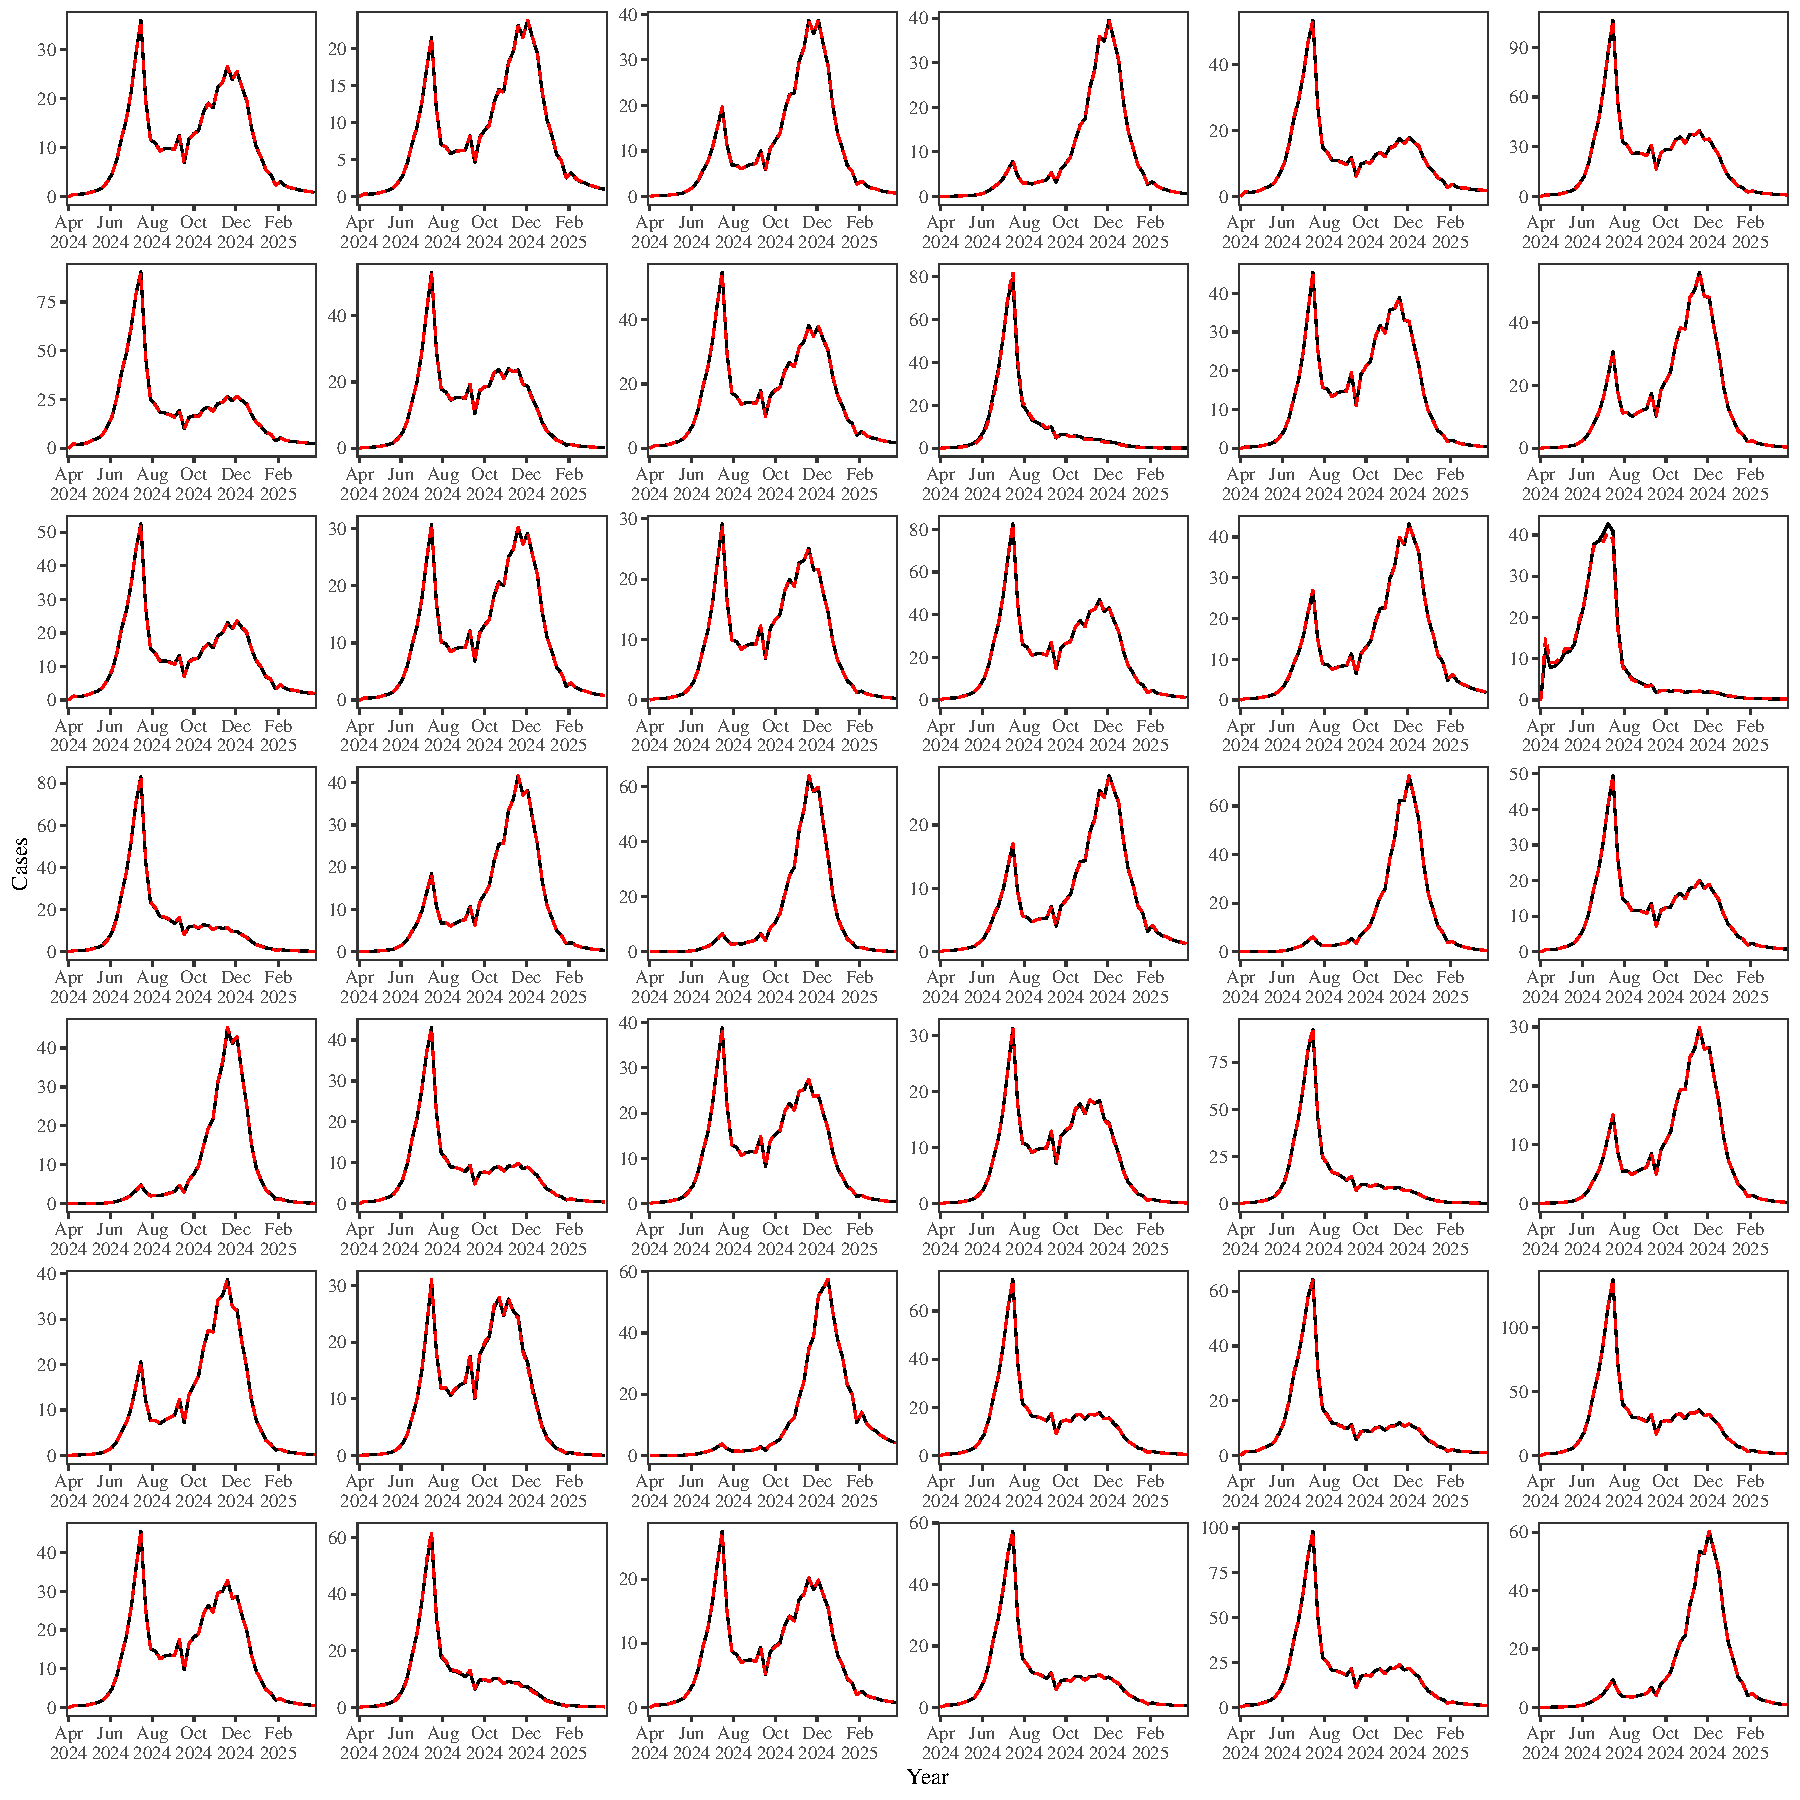
\includegraphics[width=\textwidth]{../figure/figure_compare_supp_1.pdf}
\caption{
\textbf{Comparisons between model fits across two different models.}
Solid lines represent posterior median predictions based on the model assuming separate $\mathcal R_0$ in each region.
Red lines represent posterior median predictions based on the model assuming separate $S(0)$ in each region.
}
\end{figure}

\pagebreak

\begin{figure}[!th]
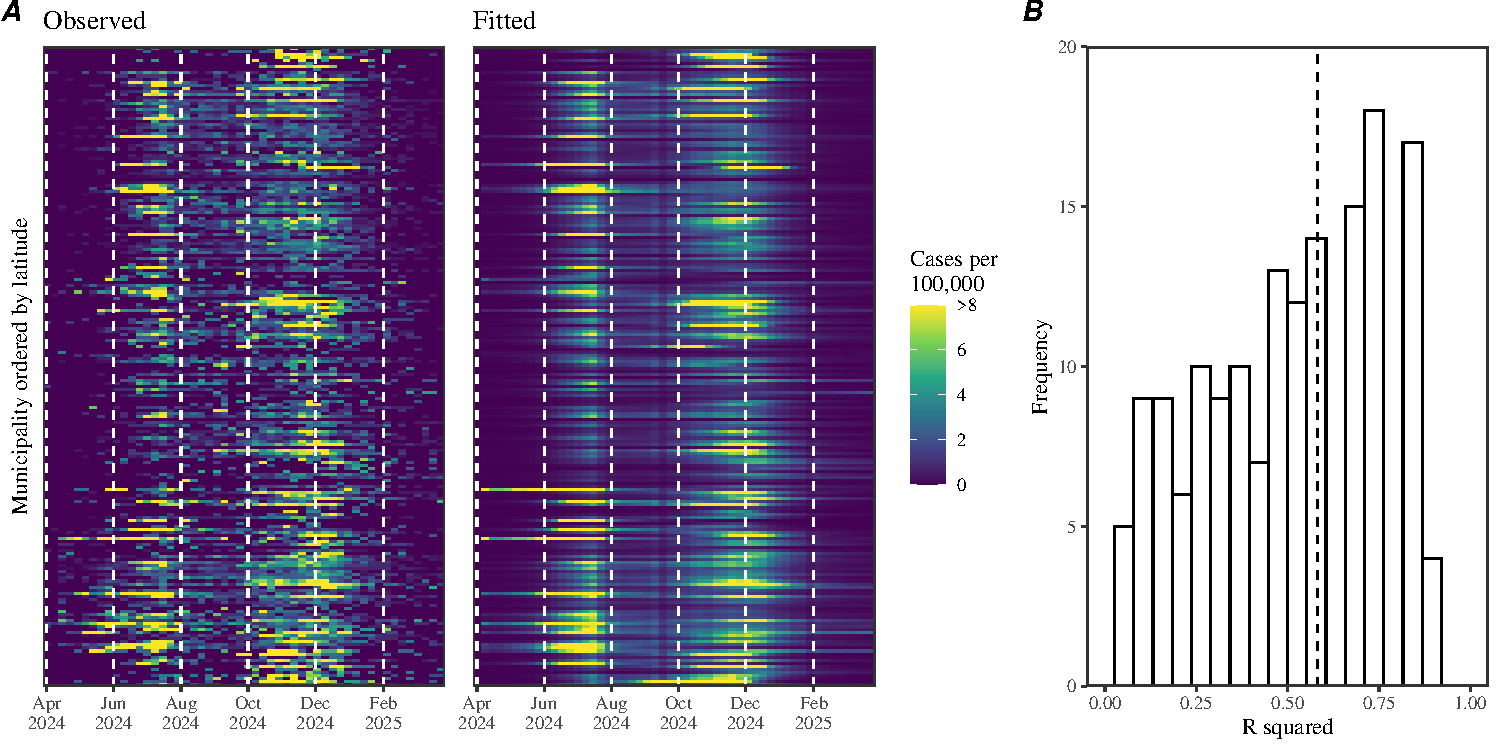
\includegraphics[width=\textwidth]{../figure/figure_stanfit_all_delta.pdf}
\caption{
\textbf{Validation of the alternative transmission model using time series data from municipalities with less than 400 total cases.}
(A) Comparisons between the observed and predicted epidemic dynamics across municipalities with less than 400 total cases, ordered by latitude.
(B) The bar plot represents the distribution of R squared values for model fits.
The vertical dashed line represents the median.
Initial infected, initial susceptible, and reporting probability were estimated for each region while assuming a known transmission variation term $\delta(t)$ and basic reproduction number.
}
\end{figure}

\pagebreak

\begin{figure}[!th]
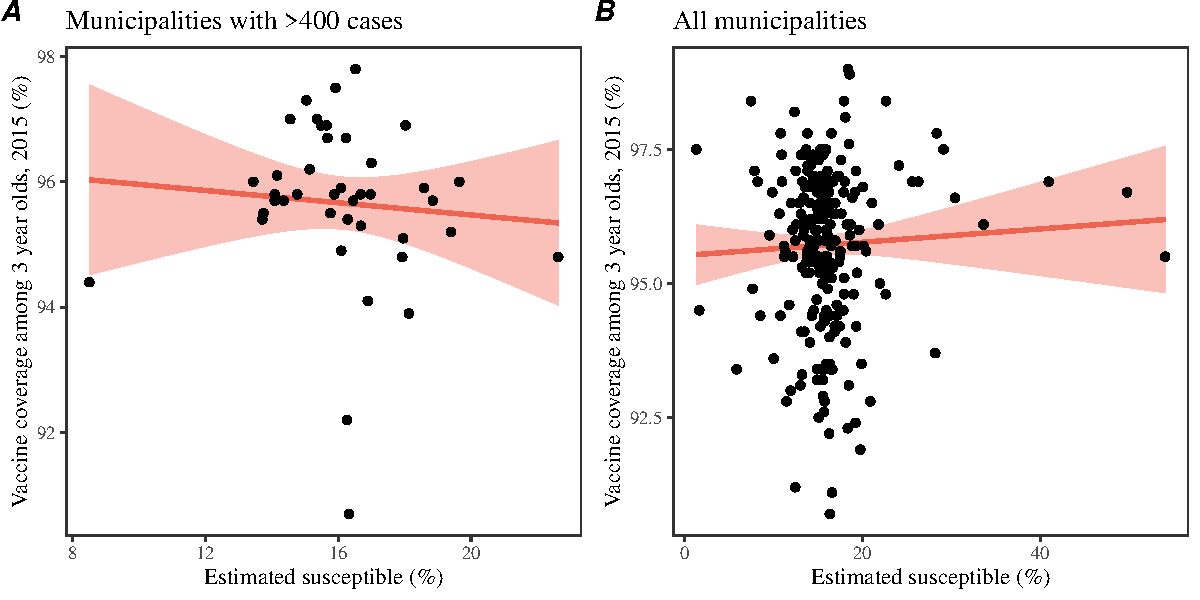
\includegraphics[width=\textwidth]{../figure/figure_stanfit_all_S0.pdf}
\caption{
\textbf{Relationship between estimated initial susceptible and vaccine coverage for (A) municipalities with $>400$ cases and (B) for all municipalities.}
Each point represents the estimate initial susceptible and vaccine coverage value for each municipality.
Red lines and shaded regions represent the linear regression fit and corresponding 95\% confidence intervals.
}
\end{figure}


\pagebreak

\bibliography{whooping-cough}

\end{document}
